\section{Model Subtree Reordering}\label{sec:msr}
In this section, we introduce our third defense mechanism (\contribution{3.3}) called \textit{model subtree reordering} (MSR)~\cite{Saglam2024a}. 
%
% MOTIVATON
Modeling assignments, such as \ac{UML} class, use case, sequence, and activity models, are common in computer science education~\cite{Ciccozzi2018, Saglam2023}. Modeling is integral to traditional software engineering courses due to the practical use of modeling languages like \ac{UML}. Furthermore, metamodeling assignments are becoming increasingly prevalent with the growing adoption of model-driven techniques~\cite{Brambilla2017, Hutchinson2011}. The complexity of modeling assignments and their demand for domain understanding and problem-solving skills make them susceptible to plagiarism~\cite{Martinez2020}. However, research on detecting plagiarism in modeling assignments is limited~\cite{Martinez2020, Saglam2022, Saglam2023}.

% REQUIREMENT: DEGREES OF FREEDOM
Effective plagiarism detection for modeling assignments necessitates mechanisms to handle degrees of freedom in models. Reordering attacks might exploit this flexible nature of models, which can lead to significant variations in the token sequence extracted from these models. While token-based detection approaches can detect large-scale reordering, for example, reordering methods in a class or classes in a \ac{UML} diagram, they are vulnerable to fine-grained reordering attacks~\cite{Saglam2022}. For program code, statements have a strong interdependence, thus limiting the effectiveness of reordering attacks (realistically, such an obfuscation attack will only reduce the similarity by about five percentage points~\cite{Saglam2024b}). For modeling artifacts, however, these fine-grained reordering attacks can effectively obfuscate plagiarism.
%
% EXAMPLE OF THIS
For example, the order of elements within multi-valued containment references can vary significantly in \ac{EMF} metamodels.
Likewise, in \ac{UML} class models, the order of attributes and methods within a class is often flexible and does not affect the model's semantics. Similarly, the sequence of states and transitions is not semantically significant in state charts. Instead, the critical aspect is the specific state from which a transition originates and the state to which it leads.
%
In the following, we discuss the targeted obfuscation attacks, the fundamental concept of model subtree reordering, the detailed algorithm, its complexity, and the limitations of the defense mechanism.

\begin{factsheet}{Overview: Model Subtree Reordering} 
    \begin{description}[style=multiline,leftmargin=5.5cm]
        \item[Core Principle] Normalize the Order of Elements in the Model
        \item[Targeted Obfuscation Attack] Model Element Reordering
        \item[Language Family] Modelling Languages
        \item[Language Dependence] Language-Agnostic
        \item[Performance Impact] Very Low
        \item[Main Scalability Determinant] Size of Input Models
        \item[Integration Complexity] Moderate
    \end{description}
\end{factsheet}

\subsection{Targeted Obfuscation Attacks}
When using token-based approaches for modeling plagiarism detection, obfuscation attacks based on moving and swapping elements on a fine-grained level pose a viable threat~\cite{Saglam2022} because of the degrees of freedom discussed above.
Consider the view on the \texttt{Store} package in \autoref{fig:example-view}. It depicts two classes with their corresponding attributes, references, and containment references.
For this model view, \autoref{tab:example-view} presents three corresponding token sequences. All three sequences correctly represent the same model elements depicted in \autoref{fig:example-view}. However, the order of tokens varies between the sequences.
The original sequence represents the element order as shown in the graphical view. The first variant is created by swapping the tokens corresponding to each class, slightly altering the token sequence. The second variant is created from the first by reordering the tokens of the features, again modifying the token sequence order completely.
%
These variations in token sequences are a form of obfuscation where the token sequence remains semantically equivalent, but its representation is altered. This is possible for \ac{EMF} or \ac{UML} models, as the order of classes in a package and the order of features in a class have no semantic relevance. This also applies to many other modeling languages. Reordering is also common in source code plagiarism, but there, it provides limited effectiveness~\cite{Saglam2024b}.

Model subtree reordering targets the unique challenges posed by ordering-based obfuscation attacks on modeling artifacts.
To reduce the impact of the degrees of freedom common in modeling artifacts, we normalize the order of tokens corresponding to the elements in the model, ensuring a consistent representation of modeling artifacts and thereby countering obfuscation efforts that rely on the fine-grained reordering elements.
However, normalization in this context is far from trivial.
The properties used for normalization must be selected carefully to avoid introducing new attack vectors, and the process must minimize changes to the token sequence to prevent false positives.
Only \textit{robust} criteria can provide stability and invariance to obfuscation attacks.

\begin{samepage}
\begin{figure}[b]
    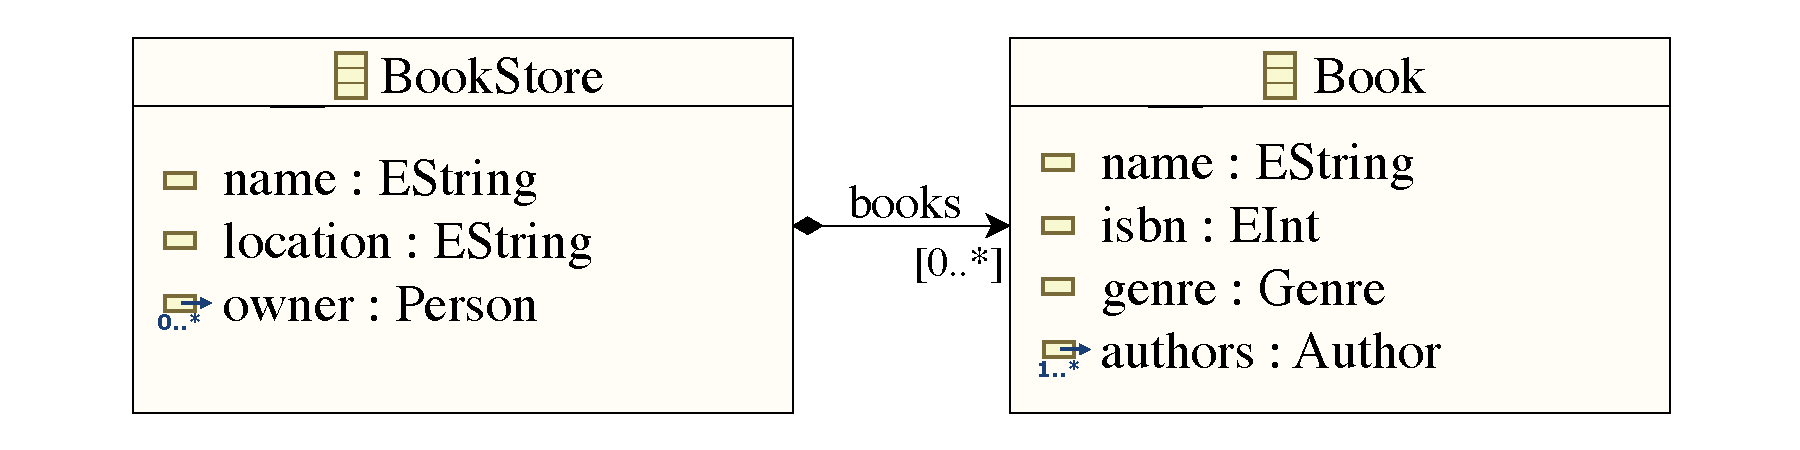
\includegraphics[width=\textwidth]{figures/mde/bookstore-view.pdf}
    \caption[Bookstore Model View]{View on the package \texttt{Store} of the second bookstore management system model as shown in \autoref{fig:running-example}, depicting two classes with their attributes and references.}
    \label{fig:example-view}
%\end{figure*}
\end{figure}

\begin{table}[b]
    \centering
    %\small
    \begin{tabular}{clll}
		\toprule
		\# & \textbf{Original}     & \textbf{Variant 1}    & \textbf{Variant 2}    \\
		\midrule
		1  & \texttt{Class}        & \texttt{Class}        & \texttt{Class}        \\
		2  & \texttt{ Containment} & \texttt{ Attribute}   & \texttt{ Attribute}   \\
		3  & \texttt{ Attribute}   & \texttt{ Attribute}   & \texttt{ Reference}   \\
		4  & \texttt{ Attribute}   & \texttt{ Attribute}   & \texttt{ Attribute}   \\
		5  & \texttt{ Reference}   & \texttt{ Reference}   & \texttt{ Attribute}   \\
		6  & \texttt{Class End}    & \texttt{Class End}    & \texttt{Class End}   \\
		7  & \texttt{Class}        & \texttt{Class}        & \texttt{Class}    \\
		8  & \texttt{ Attribute}   & \texttt{ Containment} & \texttt{ Attribute}   \\
		9  & \texttt{ Attribute}   & \texttt{ Attribute}   & \texttt{ Reference} \\
		10 & \texttt{ Attribute}   & \texttt{ Attribute}   & \texttt{ Containment}   \\
		11 & \texttt{ Reference}   & \texttt{ Reference}   & \texttt{ Attribute}   \\
		12 & \texttt{Class End}    & \texttt{Class End}    & \texttt{Class End}    \\
		\bottomrule
    \end{tabular}
    \caption[Example Obfuscation: Reordering]{Three token sequences, all representing the model view depicted in \autoref{fig:example-view}. The original reflects the element order of the view, while the first variant is created by swapping the tokens of each class, and the second variant is created from the first by reordering the tokens of the features. Note that all references are multi-valued, which is omitted for readability.}
    \label{tab:example-view}
\end{table}
\end{samepage}

Simple approaches like sorting by type or lexical order are insufficient, as they can be easily manipulated by specific obfuscation attacks (e.g., element insertion or property changes). The normalization is either ineffective or can be affected via specific obfuscation attacks.
For example, consider a hypothetical normalization based on element names: Whenever named model elements can be in an arbitrary order, they are sorted lexically via their names. While this provides resilience against reordering, it also includes vulnerability against renaming, as minor name changes now affect the element order. Besides names, other vulnerable properties include identifiers, data types, values, and other literals.
Normalization properties must be stable, invariant, and meaningful to detect plagiarism accurately and effectively.
Thus, robust properties are only based on the information already used by the plagiarism detectors and are limited to the extracted tokens corresponding to the patterns and structural patterns in these tokens.


\subsection{Concept}
As discussed in \autoref{sec:mde-approach}, tokenization references refer to the meaningful connections between elements in a model that capture the underlying semantics of the modeled system. Unlike syntactic references, which focus on the structural aspects of the model, tokenization references emphasize the relationships and dependencies that convey the intended behavior and functionality. 
Again, consider a state chart model. While structurally, all states might be contained under a common root element, these containment references are syntactic references. The underlying semantics are modeled by transition references between states, which are thus considered tokenization references.
These references are crucial for accurately detecting plagiarism in modeling assignments, as they ensure that the detection mechanisms account for the intent and semantics behind the models rather than just superficial similarities. By leveraging tokenization references, we can improve the robustness of modeling plagiarism detection. However, this also means these tokenization references must be identified for each modeling domain, as this distinction is purely conceptual and not reflected in the actual modeling artifacts.

Model subtree reordering is designed against reordering attacks by specifically leveraging these tokenization references to normalize the order of the token sequence. 
The approach applies to any modeling artifact with a tree-like structure where tokenization references can be identified. However, the effectiveness of this method depends on the extent of variability allowed within these types of artifacts.
%
To ensure a deterministic order in the token sequences representing modeling artifacts, we sort the elements in each multi-valued tokenization reference first based on their token type and then based on the distribution of the tokens in their subtree of direct and indirect children.
While the former is a coarse-grained ordering criterion to group model elements that map to the same token type, the latter is a more fine-grained one to capture and preserve the structural nuances within subtrees of the referenced elements.

At a high level, our approach leverages the concept of token type vectors to represent the structure of the model subtree. These vectors capture the frequency of various token types within the subtree, allowing us to compare and sort elements based on their structural characteristics. Thus, such a vector represents the distribution of different kinds of model elements in a specific part of the model. For example, we can consider the three subtrees illustrated in \autoref{fig:tree-examples}. Note that these are token trees, meaning the structure defined by the tokenization references of a model where each model element is replaced by its corresponding token. While all three trees are similar, subtree A has a different distribution of tokens than subtrees B and C, as each type (represented by color) occurs only once. While the subtrees B and C are structurally different, they share the same distribution of tokens. Note that the tree B can be transformed into the tree B with a single reordering operation.

If we now interpret these vectors as points in a multi-dimensional space, we can use the distance of these points to estimate how structurally similar two parts of a model are. By finding a path (meaning a sequence that includes all points) in this space that minimizes the distance between points, we can derive an order that is both deterministic and not easy to affect intentionally. This approach ensures that structurally similar elements are consistently ordered, thereby mitigating the effects of obfuscation through reordering while maintaining the stability of the normalization process.


\begin{figure}
    \centering
    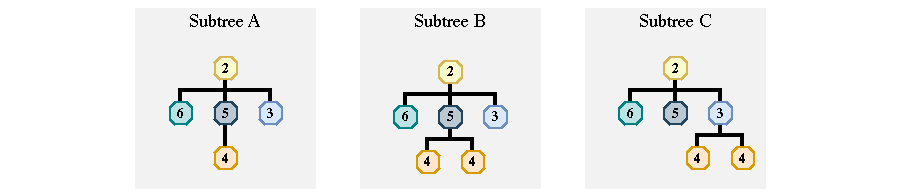
\includegraphics[width=\linewidth]{figures/mde/subtree-examples.pdf}
    \caption[Model Subtree Examples]{Three exemplary model subtrees based on tokenization references in token representation, where subtree A contains a slightly different token distribution than subtrees B and C, which share the same distribution.}
    \label{fig:tree-examples}
\end{figure}


\subsection{Algorithm}
Our normalization algorithm consists of several steps. The entire algorithm is listed in \autoref{alg:NormalizationAlgorithm}.
We begin by generating tokens for each element's subtree and then create a token type vector that indicates how often each type of token occurs within that subtree. For instance, in the case of the class \texttt{Book} depicted in \autoref{fig:tokenization}, this vector is represented as $[2, 1, 1, 0, \dots, 0]$, where the vector components correspond to two attributes, one identifier attribute, and one reference.
To enable meaningful comparisons between these vectors, we first normalize them. The normalization is done by computing the Euclidean norm of each vector:
\begin{align*}
    \|\mathbf{v}\|_2 = \sqrt{\sum_{i=1}^{n}v_i^2}
\end{align*}
This normalization process scales the vectors to have a length of 1, ensuring that the comparison between them is not influenced by the absolute magnitude of the original vectors but by the distribution of token types within each subtree.
Once normalized, these vectors can be interpreted as points in a multi-dimensional coordinate space, where each dimension corresponds to a specific token type. The position of each point in this space is determined by the distribution of token types in the corresponding element's subtree. For example, a vector with more attributes will be closer to the axis representing attributes.

To compare these points (representing different elements), we calculate the Euclidean distance between any two points $\mathbf{p}$ and $\mathbf{q}$ using the following metric:
\begin{align*}
    d_{\mathrm{E}}(\mathbf{p}, \mathbf{q}) = \sqrt{\sum_{i=1}^n (q_i-p_i)^2}.
\end{align*}
Using these distances, we construct a nearest neighbor path that sequentially connects each point to its closest neighbor, starting from the point associated with the element with the most tokens in its subtree. This ordering method prioritizes elements with greater structural complexity, which helps preserve the overall structure during the normalization process.
%
In cases where two or more points are equidistant from the last point in the path, we resolve the tie by referring to the original order of the elements. This ensures that the normalization process is stable, meaning that the same input will always produce the same normalized output, avoiding the introduction of inconsistencies due to random ordering.
%
%
Finally, to normalize the order of elements within a tokenization reference, we apply a two-step sorting process:
    \begin{enumerate}
        \item Primary Sorting by Token Type: We first sort the elements based on their token type vectors, providing a coarse-grained ordering that groups similar elements.
        \item Secondary Sorting by Nearest Neighbor Path: If two elements have identical token type vectors, we further sort them according to their position in the calculated nearest neighbor path. This fine-grained sorting helps maintain the relative order of structurally similar elements.
    \end{enumerate}
This approach ensures that the elements within a model are consistently ordered, thereby countering potential obfuscation strategies that rely on reordering elements.


\autoref{fig:tokentreenorm} illustrates the process of reordering tokens for three elements within the same (multi-valued) tokenization reference. The normed subtree vectors are used to calculate the elements' distances, sorting the elements according to the computed nearest neighbor path.
\begin{enumerate}
    \item {Token Tree}: We start with the token trees for three classes, each containing various tokens that represent different model elements such as identifiers, attributes, and references.
    \item {Subtree Vectors}: As a first step, the algorithm generates subtree vectors for each class, denoted as \( \mathbf{v}_a \), \( \mathbf{v}_b \), and \( \mathbf{v}_c \). These vectors count the occurrences of each token type within the subtrees. For example, the subtree vector for \texttt{Class} $a$ is \( \mathbf{v}_a = [1, 1, 0, \dots, 0] \), indicating one identifier and one attribute.

    \item {Normalized Vector}: Next, each subtree vector is normalized by its Euclidean norm \( \|\mathbf{v}\|_2 \). The normalized vectors represent the scaled distribution of tokens, ensuring comparability regardless of their original magnitude.

    \item {Euclidean Distance}: The normalized vectors are then used to calculate the Euclidean distance between each pair of elements. The distance matrix \( D \) encapsulates these distances, with each entry \( d_{ij} \) representing the distance between the vectors of \texttt{Class} $i$ and \texttt{Class} $j$. For example, the distance between \( \mathbf{v}_a \) and \( \mathbf{v}_b \) is \( d_{ab} = 0.765 \).

    \item {Nearest Neighbor Path}: Using the distance matrix \( D \), the algorithm determines the nearest neighbor path. The path starts from the element with the largest subtree (in this case, \texttt{Class} $b$) and proceeds by selecting the nearest neighbor at each step.

    \item {Normalized Token Sequence}: Finally, the model elements are reordered according to the nearest neighbor path, resulting in a normalized token sequence.
\end{enumerate}


\begin{figure}
    \centering
    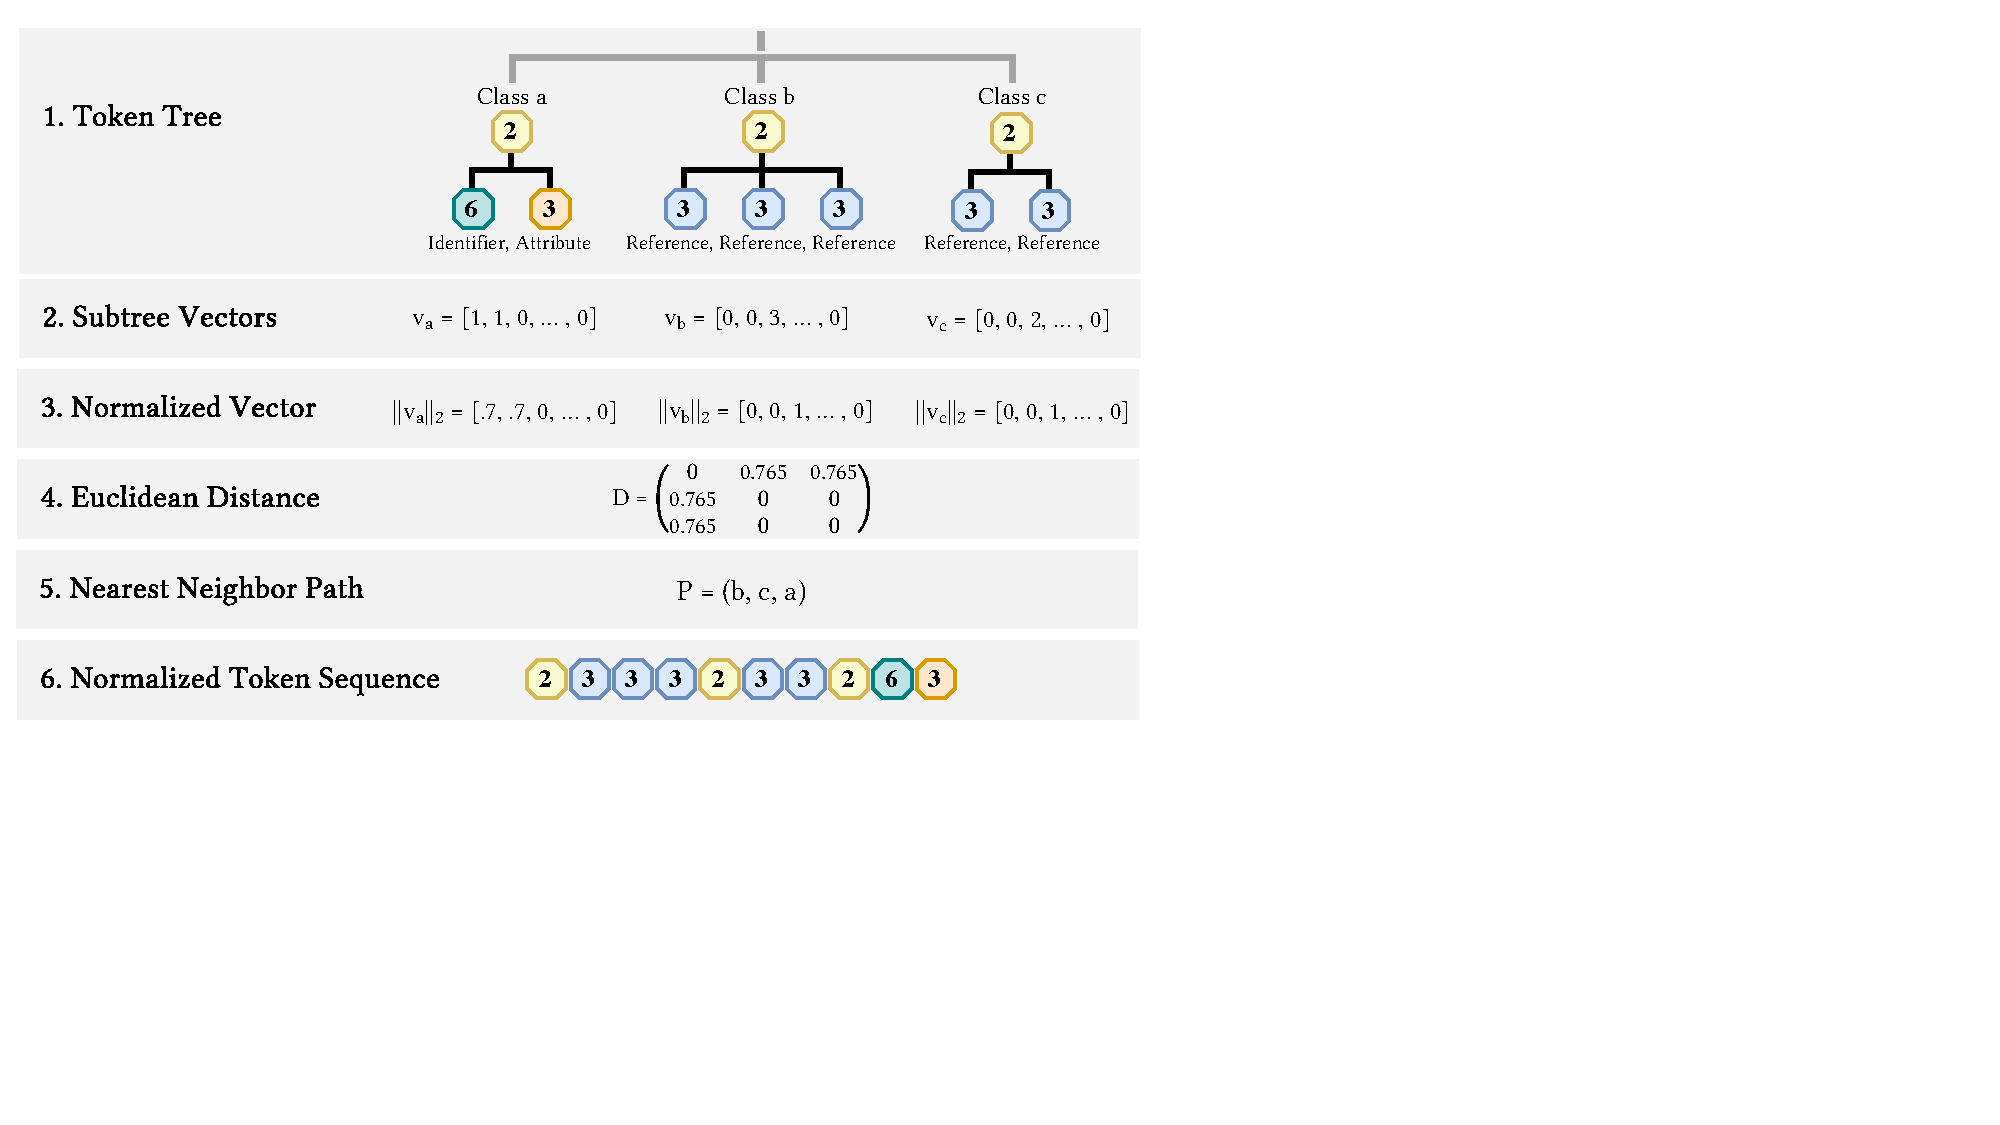
\includegraphics[width=0.9\linewidth]{figures/mde/normalization-new.pdf}
    \caption[Model Subtree Reordering Example]{Example illustrating how model subtree reordering normalizes the token sequence via element reordering for a multi-valued reference containing three classes.}
    \label{fig:tokentreenorm}
\end{figure}

\begin{algorithm}
    %\captionsetup{belowskip=-\baselineskip}
	\caption{Model Subtree Reordering}
	\label{alg:NormalizationAlgorithm}
	\begin{algorithmic}
		\Require{List of model elements $E$ with length $n$}
		\Function{Normalize Token Sequence}{$E$}
		\State{$V \gets$ empty list of vectors}
        \For{$e_i \in E$}
		      \State{$v_i \gets$ calculate token type vectors for subtree of $e_i$}
            \State{$v_i \gets$ euclidean norm $\|\mathbf{v_i}\|_2 $}
		\EndFor
  
        \State{$D \gets$ empty distance matrix with size $n \times n$ }
		\For{$v_i, v_j \in V$}
		      \State{$d_{i,j} \gets$ euclidean distance $d_{\mathrm{E}}({v_i}, {v_j})$}
		\EndFor
  
		\State{$v_{max} \gets$ vector in $V$ of element with largest subtree}
            \State{$P \gets$ nearest neighbor path for $D$ starting from $v_{max}$}
            \State{$S \gets$ sort $E$ by token type, if equal by position in $P$}
            \State{\Return{$S$}}
		\EndFunction
	\end{algorithmic}
\end{algorithm}

% OLD VERSIONS
%\input{tables/normalization}

\noindent

In our approach, we opted to use the nearest neighbor path rather than the shortest path, as the nearest neighbor path is more robust against modifications in the subtrees. The shortest path, which typically minimizes the total distance between points in a coordinate space, can be sensitive to even minor changes in the structure of the elements, potentially leading to significant shifts in the ordering. Such sensitivity would make the normalization less robust.

On the other hand, the nearest neighbor path focuses on maintaining local consistency by linking each point to its closest neighbor, regardless of the overall path length. This method ensures that small changes in the subtree structure do not disproportionately affect the overall sequence, making the path, and hence the normalization, more resilient to obfuscation techniques that involve subtree modifications.

We further enhance the robustness of the normalization by carefully choosing the starting point for constructing the nearest neighbor path. Specifically, we start from the element with the most tokens in its subtree. This choice is based on findings from our pre-study, which indicated that beginning with the most complex (or structurally significant) element leads to a normalization more resistant to reordering attacks. The rationale is that the element with the most tokens likely has a more pronounced impact on the overall model structure, making it a stable anchor for the normalization process.

Using the nearest neighbor path and selecting a strategic starting point, our approach effectively addresses the normalization challenge in modeling plagiarism detection. It ensures that similar structures are consistently ordered in a way that is less susceptible to manipulation. This combination of strategies—prioritizing local consistency and starting with the most significant element—provides a more stable and reliable method for detecting plagiarism in models.


\subsection{Complexity}
The runtime complexity of the model subtree reordering algorithm in \autoref{alg:NormalizationAlgorithm} depends on the tree defined by the tokenization references and is thus influenced by the size of the subtrees and the number of model elements. Note that a tree with $m$ nodes can have a maximum of $m$ subtrees when every node except the root is a leaf. Furthermore, the maximum number of tokens in a subtree is limited by $m$.

The runtime complexity of model subtree reordering depends on the three main operations: Calculating the token type vectors, computing the distance matrices, constructing the distance matrices, and sorting the subtrees via a nearest neighbor search.
%
For an entire model of $m$ elements, the token type vectors for each subtree can be calculated via a single depth-first search with the runtime complexity of $O(m)$.
Constructing the distance matrix involves computing pairwise distances for up to $m-1$ elements (when all model elements are leaves of a single root), which contributes $O(m^2)$ complexity.
Sorting of all elements according to their distances via a nearest neighbor search has a complexity of $O(m \log m)$.

The overall runtime complexity is thus $O(m^2)$.
As the worst-case runtime complexity for greedy string tiling per program pair is \( O(m^3) \) (see \autoref{sec:found-jplag}), model subtree reordering does not increase the runtime complexity of the plagiarism detection process.

\subsection{Limitations}\label{sec:msr-limits}
While model subtree reordering is a robust defense mechanism against reordering-based obfuscation attacks for modeling artifacts, it does have certain limitations. In the following, we discuss its dependence on tokenization references, the focus of the defense mechanism, and the effect on unrelated models.

%\begin{enumerate}
    \subsubsection{Dependence on Identifying Tokenization References} As our general approach to modeling plagiarism detection, model subtree reordering 
    depends on the modeling domain and language (see \autoref{sec:mde-limit-domain}). Model subtree reordering operates on stable tokenization references to establish a normalized order. For tree-based models like \ac{EMF} models or \ac{UML} class models, these tokenization references are the containment relations. However, identifying these references is not trivial for some modeling languages and may require domain-specific adjustments for different modeling languages (see \autoref{subsec:tokenization}). This dependency on domain knowledge limits the mechanism as it increases the complexity of applying it to new modeling languages. Nevertheless, this domain-specific adjustment is required to apply our detection approach in the first place and is, thus, no additional effort for model subtree reordering.
    
    \subsubsection{Focused Resilience} model subtree reordering is designed to mitigate reordering attacks by normalizing the token sequence based on model element distributions in subtrees. However, it does not provide resilience against other forms of obfuscation, such as inserting irrelevant model elements. %Such attacks can introduce variability that model subtree
    Although model subtree reordering leverages token subtree distributions, which are much more robust than simpler, vulnerable criteria (e.g., names), substantial modifications to specific parts of a model can still impact the normalization. Such modifications would require significant changes, such as inserting entirely new subtrees, rather than minor adjustments, like adding individual elements. The reason for this is the sorting via nearest neighbor paths, which is not affected by minor changes to the token vectors.
    Even with these large-scale modifications, the effect on obfuscation may remain limited, as inserting new subtrees only partially disrupts the ordering.
    To address cases where the normalization provided by model subtree reordering is affected, model subtree reordering can be combined with subsequence match merging, which combines focused and broad resilience.

    \subsubsection{Effect on Unrelated Models}
    Another limitation of model similarity reordering is that any normalization process can inadvertently increase the similarity of unrelated models. As a normalization technique seeks to resolve ambiguities and standardize representations, it may lead to a situation where models that initially exhibit different structures appear more similar due to the reordering.
    As for all normalization techniques, the question with model subtree reordering is how pronounced this effect is.
    As token subtree reordering is a very abstract technique that only considers the tokens themselves to limit itself to a robust normalization criterion, its normalization of the token order is very broad. In contrast, token sequence normalization only reorders tokens of statements that are not interdependent. Model subtree reordering generally reorders all model elements for each tokenization reference. Thus, it may also affect unrelated models.
    This issue may be less significant for larger models, as they generally produce larger token subtrees with a more complex token distribution. This complexity results in more unique vectors for reordering based on the nearest neighbor paths. In contrast, smaller models do not benefit from this complexity, making the effects of normalization on unrelated models potentially more pronounced.
  